\documentclass{amsart}
\usepackage{amsmath}
\usepackage{graphicx}

% hyperref
\usepackage[bookmarks=true, linktocpage=true,
bookmarksnumbered=true, breaklinks=true,
pdfstartview=FitH, hyperfigures=false,
plainpages=false, naturalnames=true,
colorlinks=true, pagebackref=true,
pdfpagelabels]{hyperref}
\hypersetup{
	colorlinks,
	citecolor=blue,
	filecolor=blue,
	linkcolor=blue,
	urlcolor=blue
}

% layout
\setlength{\textwidth}{\paperwidth}
\addtolength{\textwidth}{-1.85in}
\setlength{\textheight}{\paperheight}
\addtolength{\textheight}{-2in}
\calclayout

% Updating to MSC2020
\makeatletter
\@namedef{subjclassname@2020}{%
	\textup{2020} Mathematics Subject Classification}
\makeatother

% Commands
\renewcommand{\S}{\mathrm S}
\renewcommand{\P}{\mathrm P}
\DeclareMathOperator{\trace}{Trace}
\DeclareMathOperator{\init}{Init}
\DeclareMathOperator{\term}{Term}

% Revision
\newcommand{\rev}[1]{\textcolor{red}{#1}} % red/black

\begin{document}
	
\title{Homotopy coherent symmetries for the permutahedral diagonal}
\author{Anibal M. Medina-Mardones}
\address{Max Plank Institute for Mathematics, Bonn, Germany}
\email{ammedmar@mpim-bonn.mpg.de}
\address{Department of Mathematics, University of Notre Dame, Notre Dame, IN, USA}
\email{amedinam@nd.edu}
\thanks{The author acknowledges financial support from Innosuisse grant \mbox{32875.1 IP-ICT - 1}.}
\keywords{.}
\subjclass[2020]{.}

\begin{abstract}
	
\end{abstract} 

\vspace*{-1cm}

\maketitle

\section{Introduction}

\section{Permutahedra}

Consider the symmetric group $\S_n$ with $n$ elements together with $G$, the preferred ordered set of generators $\tau_i = (i, i+1)$ for $i \in \{1,\dots,n-1\}\}$.
Let us consider the Cayley graph of the associated presentation.
We can regard this as the 1-skeleton of a CW-complex $\P_n$, see Figure \ref{f: cayley s4}.
Its faces correspond to cosets of subgroups generated by subsets of $G$.

\begin{figure}[!h]
	\begin{equation*}
	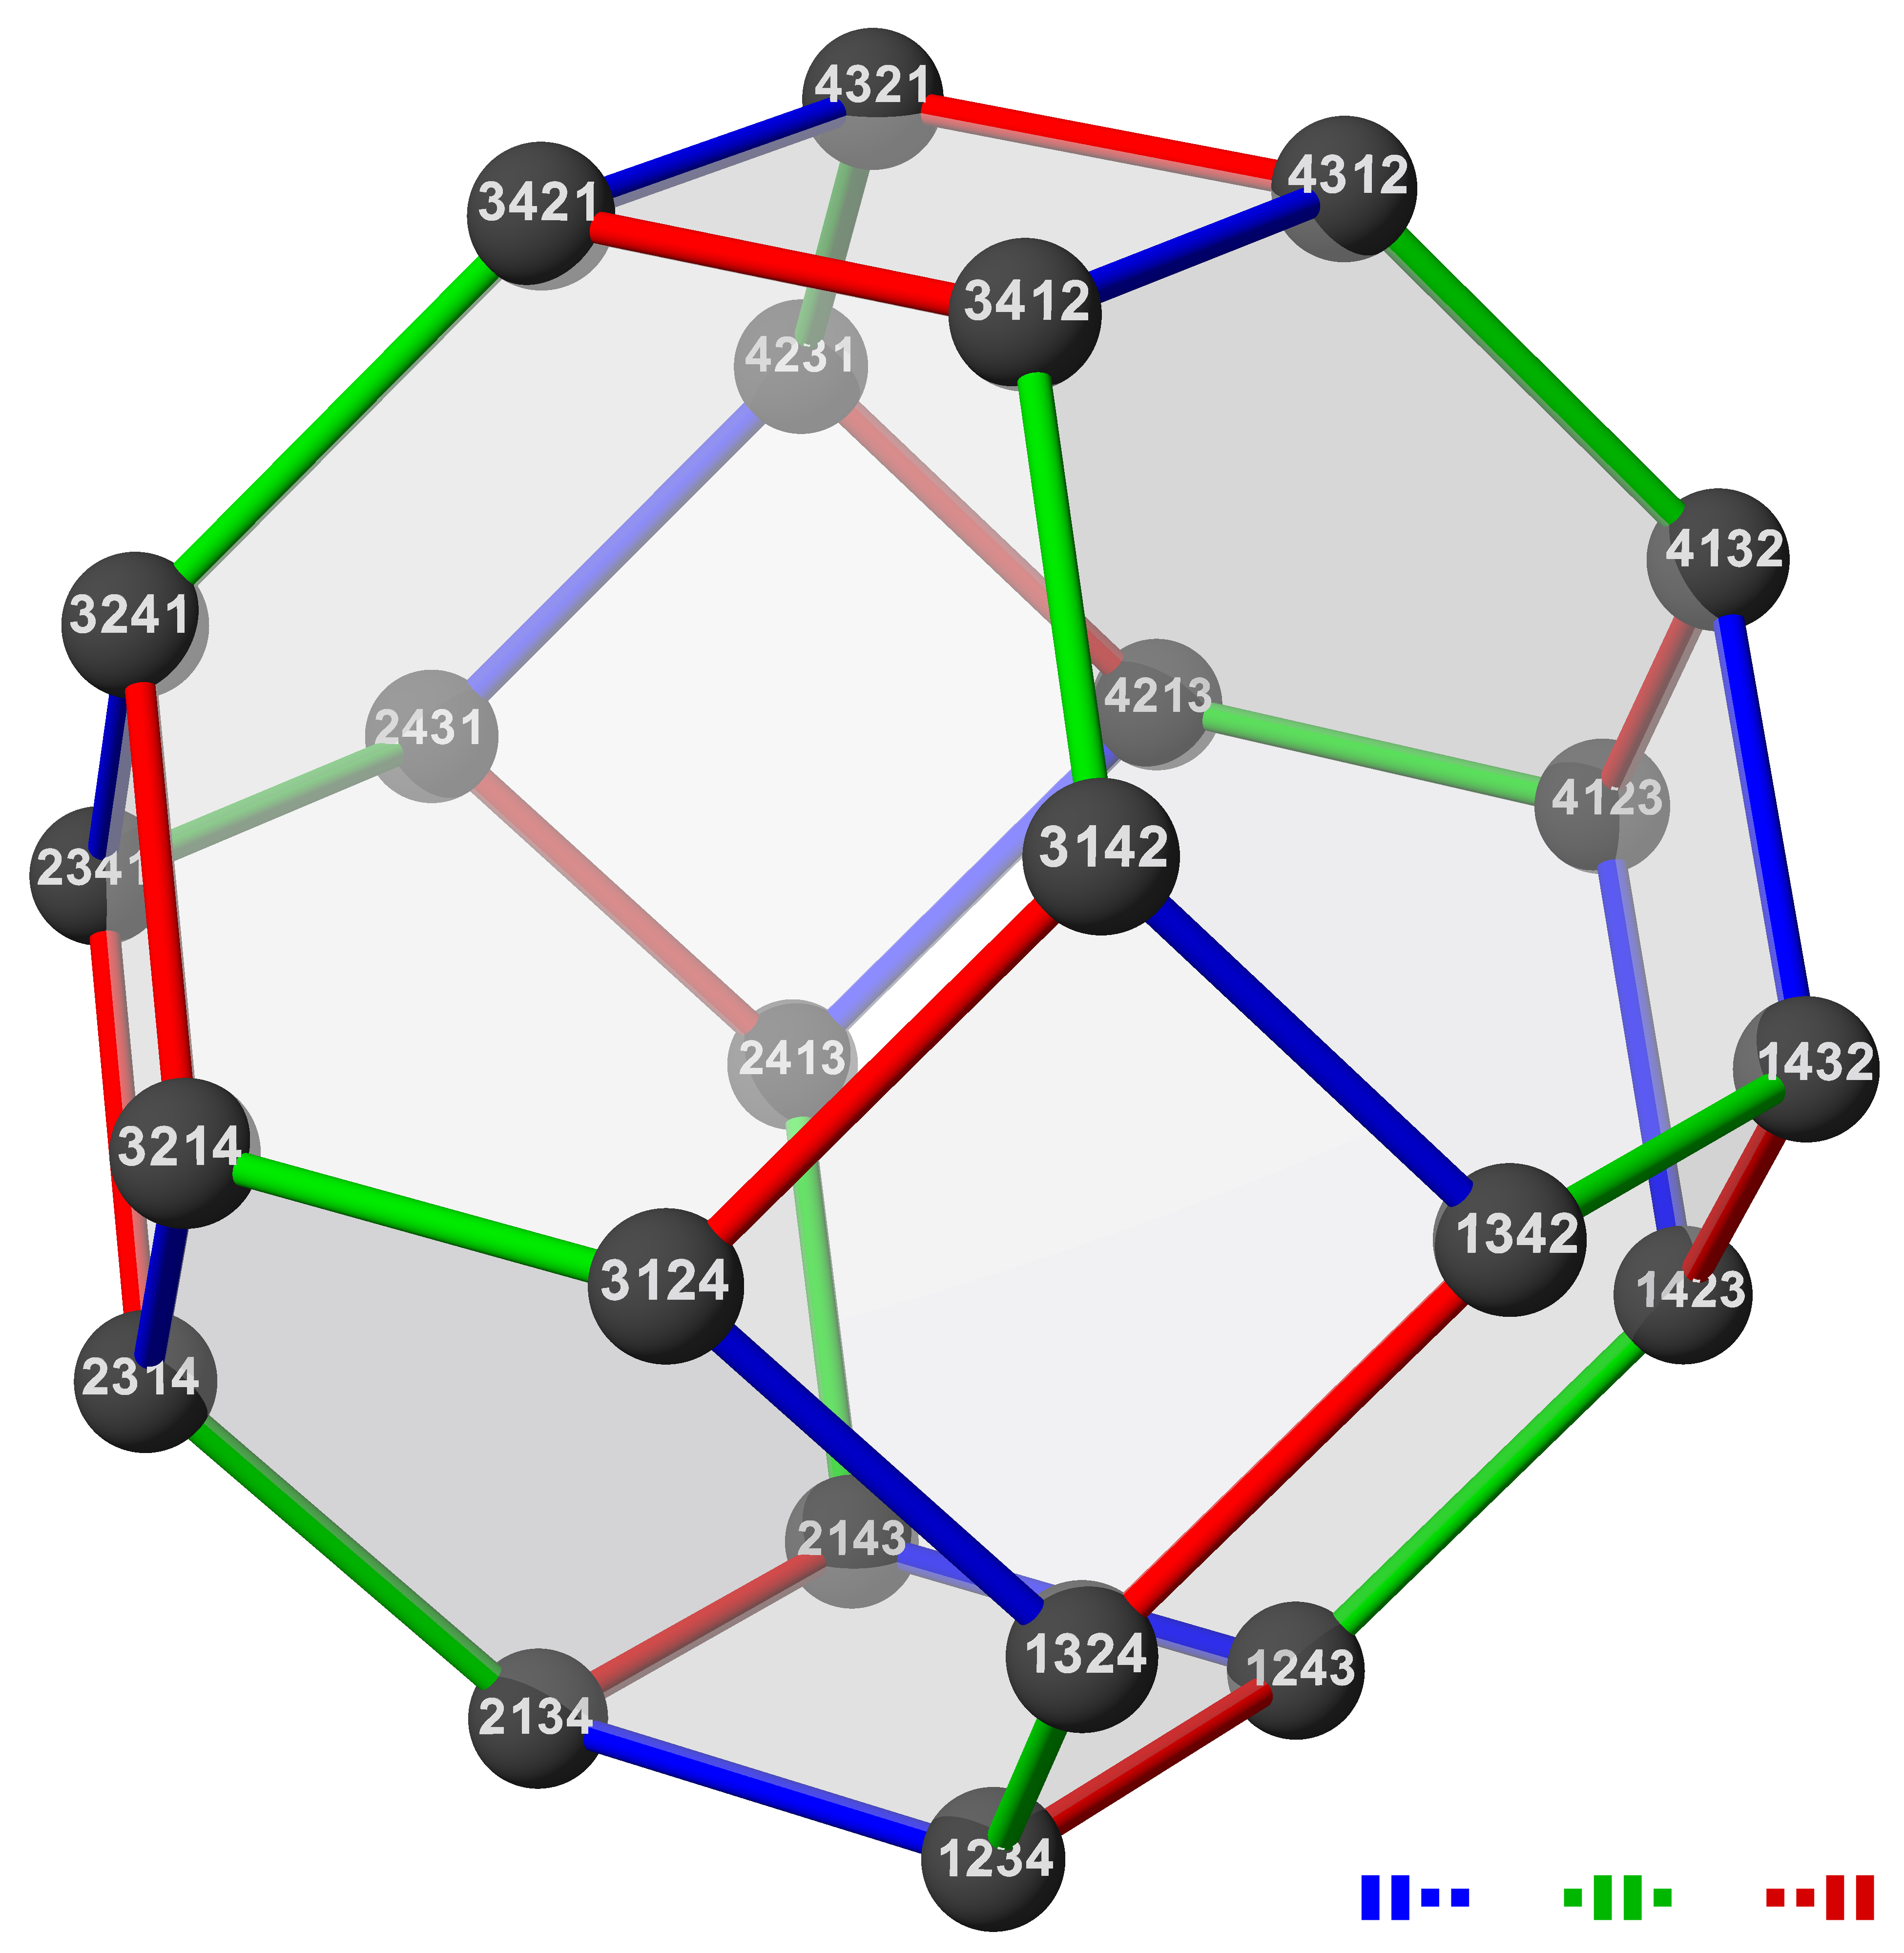
\includegraphics[scale=.07]{figures/cayley_s4.png}
	\end{equation*}
	\caption{$\P_4$}
	\label{f: cayley s4}
\end{figure}

There is a natural partial order on $\S_n$.
A (left) inversion in a permutation $\sigma \in \S_n$ is a pair of values $1 \leq i < j \leq n$ such that $\sigma^{-1}(i) > \sigma^{-1}(i)$, i.e. $i$ appears after $j$ in $(\sigma(1), \dots, \sigma(n))$.
The (right) poset structure on $\S_n$ is the partial order induced from inclusion of sets of inversions.
Notice that $\S_n$ has a minimal and maximal element with respect to this order, we denote them $\underline{0} = (1, \dots, n)$ and $\underline{1} = (n, \dots, 1)$ respectively.
An interval in $\S_n$ is a subset of the form
\begin{equation*}
[\sigma, \sigma^\prime] = \{\sigma^{\prime\prime}\ |\ \sigma \leq \sigma^{\prime\prime} \leq \sigma^\prime\}.
\end{equation*}

Given $\sigma \leq \sigma^\prime$ in $\S_n$, the set of \textit{paths} from $\sigma$ to $\sigma^\prime$, denoted $\Omega(\sigma, \sigma^\prime)$, consists of all sequences $(\tau_{s_1}, \dots, \tau_{s_m})$ of generators such that $\sigma^\prime = \tau_{s_n} \cdots\ \tau_{s_1} \sigma$. 

\textit{Claim}: All ascending paths have the same length.

Let $m$ be the length of paths from $\sigma$ to $\sigma^\prime$.
An integer $k \in \{0, \dots, m\}$ is said to be a \textit{junction} of $\Omega(\sigma, \sigma^\prime)$ if the element $\tau_{s_k} \cdots\ \tau_{s_1} \sigma$ is the same for any path $(\tau_{s_1}, \dots, \tau_{s_m})$ in $\Omega(\sigma, \sigma^\prime)$.
We refer to this element as the \textit{value} of the junction.
Notice that $0$ and $m$ are junctions with values $\underline{0}$ and $\underline{1}$ respectively.

\textit{Claim}: Given a pair of consecutive junctions of $\Omega(\sigma, \sigma^\prime)$ with values $\rho$ and $\rho^\prime$, the interval $[\rho, \rho^\prime]$ is a face of $\P_n$ whose dimension is the length of a path from $\rho$ to $\rho^\prime$.

Given $\sigma \in \S_n$, consider $\Omega(\underline 0, \sigma)$ and $\Omega(\sigma, \underline 1)$. We refer to the faces defined by junctions in these path sets as \textit{initial} and \textit{terminal} respectively denoting the sets containing them by $\init(\sigma)$ and $\term(\sigma)$.

%Thinking of an ascending path geometrically as a set of edges, its trace is the set of vertices it contains, explicitly $\trace(\tau_{s_1}, \dots, \tau_{s_m}) = \{\sigma, \tau_{s_1}\sigma, \dots, \sigma^\prime\}$.
%
%For any $\sigma \in \S_n$ consider the 

%Given an element $\sigma \in \S_n$, the  The order on $G$ determines a 


\newpage

\bibliographystyle{ieeetr} % ieeetr
\bibliography{bibliography}

\end{document}